\chapter{Marco Conceptual y Estado de la técnica} \label{chp:technique-state}

En este capítulo se hará hincapie en conceptos propios de la renderización \textit{2D} \ref{sec:fundations-2d}, tales como el \textit{antialiasing} \ref{subsec:antialiasing}, y en el estado de la técnica existente: \textit{APIs} más utilizadas \ref{sec:apis-render} y software que los implementa \ref{sec:current-implementations}, así como las características más distintivas de estos motores, como podría ser la personalización de \textit{shaders} en \textit{Godot} \ref{par:shaders-godot}.

\section{Fundamentos de Renderización 2D} \label{sec:fundations-2d}

\subsection{Antialiasing} \label{subsec:antialiasing}

Esta técnica es fundamental para evitar el denominado \textit{aliasing} \cite{webVulkanAntialiasing} y conseguir gráficos sin ruido y suaves. El \textit{aliasing} es un término acuñado del procesamiento de señales, que ocurre en la digitalización de las señales analógicas en las que la frecuencia de muestreo es inadecuada; esta frecuencia es llamada \textit{sampling rate}. Si se analiza la señal con una frecuencia baja, el resultado difiere gravemente de la señal original y resulta en cambios de color abruptos y erróneos. El método para evitar esta distorsión es evidente: aumentar el \textit{sampling rate}; aunque evidente, su coste es alto.

En el contexto de gráficos y renderizado 2D, las formas primitivas serían el mundo analógico descrito matemáticamente que se representan digitalmente en píxeles discretos en una pantalla. Crea el mismo efecto, pues existe un elemento analógico, siendo aquí una línea descrita matemáticamente, y un elemento digital, siendo este un píxel discreto. El \textit{sampling rate} en este caso sería la cantidad de muestras que se toman en cuenta para cada píxel, y cuantas más muestras se tomen, el color final será más cercano al ideal matemático del que se parte. Una manera fácil de entenderlo es imaginar una línea que pasa por un conjunto de cuadrados diagonalmente y entender que se formaría una cantidad abundante de esquinas, en forma de escalera, que dejarían la geometría abrupta y rugosa.

Una técnica simple y efectiva es el \textit{supersampling}. Consiste en renderizar la imagen a una mayor resolución para que cada pixel obtenga sus datos de múltiples \textit{sample} . De esta forma, algunos píxeles que antes no se tomarían en cuenta ahora se procesan y se suaviza la forma; el color obtenido por estos píxeles cuyas muestras no son completamente cubiertas se verá alterado y difuminado para conseguir este efecto de suavidad, pues el píxel toma el color promedio de sus \textit{sample} . Es una técnica cara en tiempo de ejecución, aunque funciona.

Esta idea se puede expandir y mejorar: \textit{multisampling}. Es una modificación del \textit{supersampling} en la que la idea es la misma, aunque la frecuencia con la que se ejecuta el \textit{fragment shader}, o \textit{FS}, es menor que el número de \textit{samples} por píxel; es común un ratio 4:1.

En la figura \ref{fig:comparison-aliasing} se compara un mismo modelo con y sin \textit{antialiasing.}

\begin{figure}[htp]
    \centering
    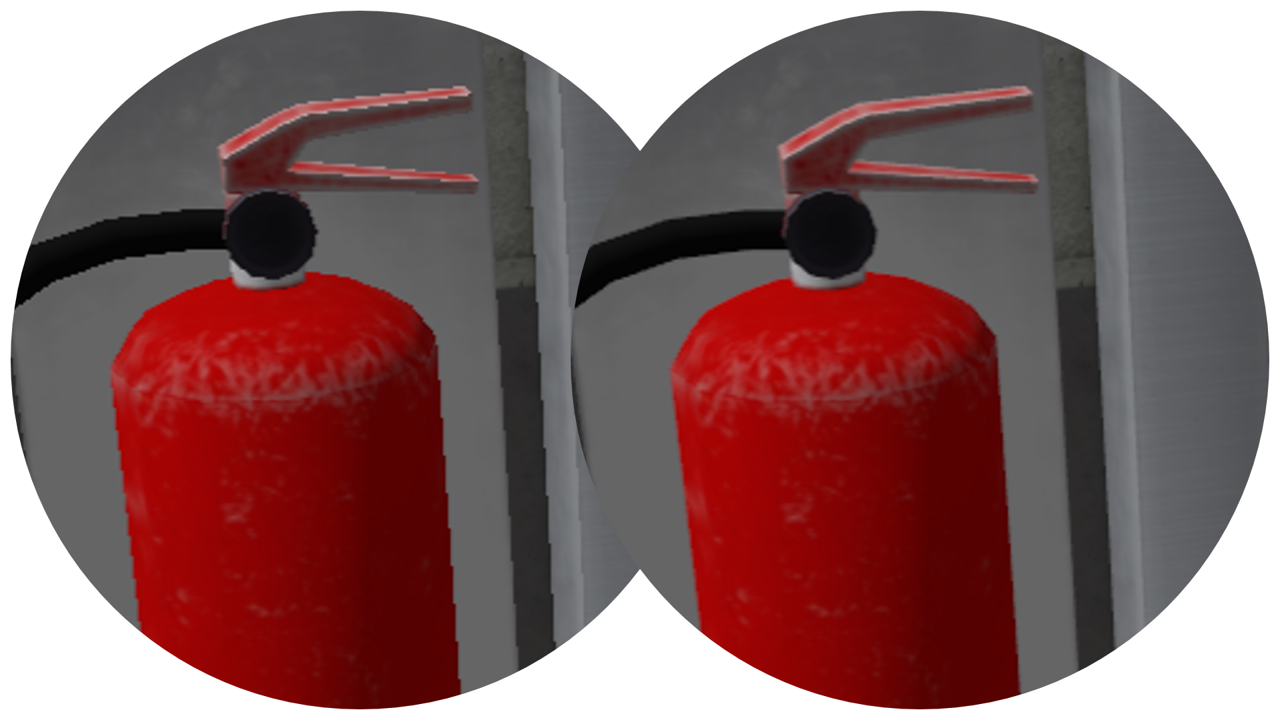
\includegraphics[width=1.0\textwidth]{figures/example_comparison_aliasing.png}
    \caption{Comparación de dos modelos, uno sin antialising y otro con antialiasing.}
    \label{fig:comparison-aliasing}
\end{figure}

En la figura \ref{fig:triangle-no-msaa} puede observarse cómo se evalúan los píxeles de un simple triángulo, quedando unos ``escalones'' muy prominentes. En la figura \ref{fig:triangle-msaa} se utiliza \textit{antialiasing MSAA}, en la que se suavizan los bordes alterando el color ligeramente.

\begin{figure}[htp]
    \centering
    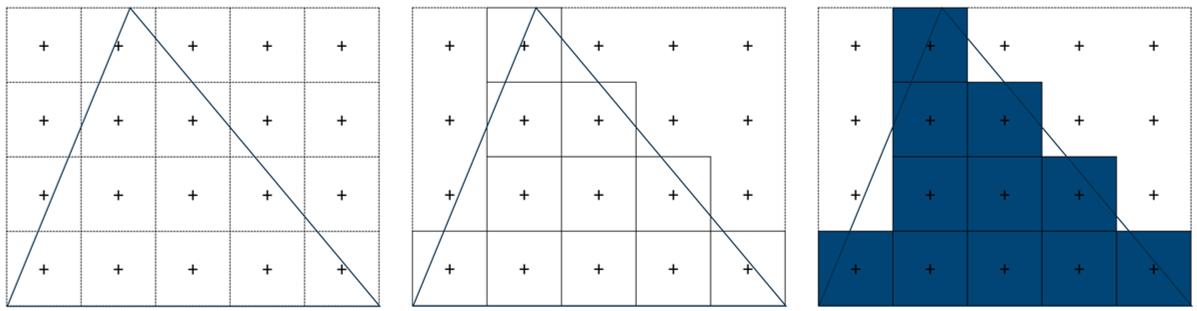
\includegraphics[width=1.0\textwidth]{figures/steps_no_msaa.png}
    \caption{Colores de un triángulo siendo evaluados sin antialiasing.}
    \label{fig:triangle-no-msaa}
\end{figure}

\begin{figure}[htp]
    \centering
    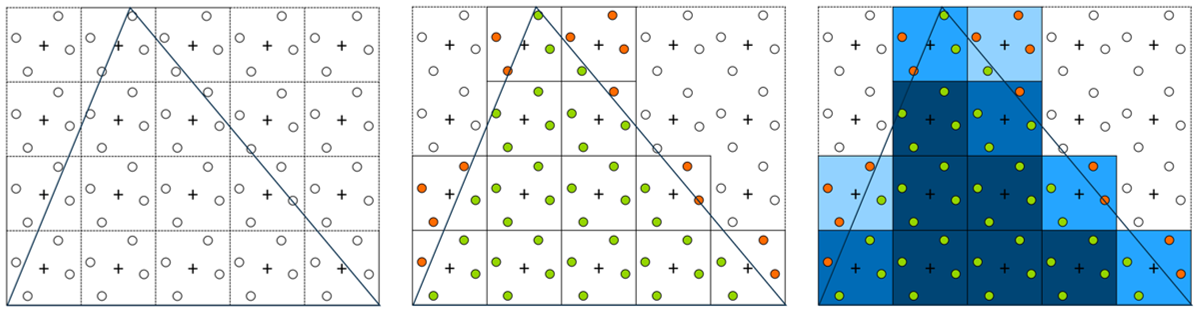
\includegraphics[width=1.0\textwidth]{figures/steps_msaa.png}
    \caption{Colores de un triángulo siendo evaluados con antialiasing MSAA}
    \label{fig:triangle-msaa}
\end{figure}

\section{APIs de Renderización} \label{sec:apis-render}

Entre las APIs de renderizado, destacan \textit{OpenGL} \cite{webKhronosOpenGL} y \textit{Vulkan} \cite{webKhronosOpenGL}, ambas desarrolladas por \textit{Khronos} \cite{webKhronos}. De hecho, \textit{OpenGL} es la predecesora de \textit{Vulkan} y se mantiene como una opción estable y sencilla de utilizar. 
Aunque \textit{Vulkan} es mucho más flexible, introduce complejidad; concretamente, está dirigido a aplicaciones muy demandantes que necesitan maximizar la eficiencia \cite{webNvidiaOglVulkan}.

\section{Implementaciones existentes} \label{sec:current-implementations}
Antes de abordar el desarrollo de un renderizador, ha sido necesario documentar sobre el funcionamiento de otros motores existentes, de forma que, aunque el propósito sea diferente, el análisis se ha centrado en las partes relacionadas con el proyecto. Cabe destacar que algunos motores, como \textit{Unity} o \textit{Unreal Engine}, son de software privativo y no pueden diseccionarse al detalle como podría hacerse con \textit{Godot}; en este caso, la única documentación disponible es el manual de usuario.

\subsection{Godot}

Renderización 2D \cite{webGodot2DRendererDocs} y 3D \cite{webGodot3DRendererDocs} acompañado de un motor de física. Incluye \textit{tilemaps}, partículas y animaciones. Se centra en luces, sombras, movimiento de partículas y visualización de \textit{meshes}. Usa \textit{OpenGL}, \textit{DirectX} y \textit{Vulkan} como \textit{APIs} de gráficos. Usa optimización \textit{GPU}. 

\paragraph{Luces y sombras}
Al igual que el resto del motor, las mecánicas de iluminación consisten en \textbf{nodos} o \textbf{vértices} en un grafo. Por ejemplo, \textit{DirectionalLight2D} \cite{webGodotDL2D} es usado para modelar la luz del sol o de la luna, \textit{CanvasModulate} \cite{webGodotCM} para dar color a la luz y, el elemento más común, \textit{PointLight2D} \cite{webGodotPL2D}, que es un punto de luz que podría ser una antorcha, fuego, proyectiles o similar. Para modelar sombra, se puede usar \textit{LightOccluder2D} \cite{webGodotLO2D}, indicando al \textit{shader} qué parte de la escena debe contener sombras.

\paragraph{2D Meshes}
Aunque menos usadas que los modelos \textit{3D}, dado que las imágenes son usadas con más frecuencia, \textit{Godot} da completo soporte a los modelos bidimensionales. También, es posible visualizar modelos tridimensionales a través de algunas herramientas en una escena de dos dimensiones. Permite convertir imágenes \textit{Sprite2D} \cite{webGodotSprite2D} a modelos 2D \textit{MeshInstance2D} \cite{webGodotMI2D}, ajustando parámetros según la calidad y rapidez que se requiera; puede ser mejor renderizar un modelo a partir de una imagen que directamente visualizar la imagen, especialmente con imágenes grandes, dibujando sólo las partes opacas e ignorando el resto

\paragraph{Animación 2D}
Hay dos formas de crear animación en dos dimensiones: a través de \textit{AnimatedSprite2D} \cite{webGodotAS2D}, una manera sencilla que sólo involucra cambio de textura, y \textit{AnimationPlayer} \cite{webGodotAP}, una manera más compleja que permite realizar más acciones en la animación, como reproducir sonidos, activar y desactivar \textit{hitboxes} \cite{webValveHitbox}, y demás. Se suele usar una plantilla de imágenes llamada \textit{sprite sheet} que recopila la animación en una sóla imagen, en vez de crear imágenes individuales para cada estado.

\paragraph{Antialiasing 2D}
Ofrece ajustes sobre el \textit{antialising} generales. Para las líneas puede activarse sin necesidad de \textit{MSAA}. Si se quiere utilizar el efecto sobre cualquier otra geometría, es necesario activar \textit{MSAA 2D} \cite{webGodotMSAA2D} en los ajustes del proyecto.

\paragraph{Shaders} \label{par:shaders-godot}
\textit{Godot} permite el uso de \textit{shaders} personalizados, con un lenguaje semejante \cite{webGodotShadingLanguage} a \textit{GLSL}, el lenguaje de \textit{OpenGL}. Los \textit{shaders} deben estar vinculados a un \textit{Material} \cite{webGodotMaterial} y este a un \textit{objeto}. Para interactuar con el \textit{shader} desde el código, se usan \textit{uniform}, de forma semejante a \textit{GLSL}, excepto que las funciones son propias del motor, como es \textit{set\_shader\_parameter}, indicando simplemente el nombre y el valor a actualizar, y \textit{get\_shader\_parameter} que recupera el valor de una variable indicando el nombre. Ambas funciones se definen en la clase \textit{Material}.
    
\subsection{Blender}
Renderización 2D y 3D. Tiene tres renderizadores, aunque el más relevante es \textit{Cycles} \cite{webBlenderCyclesDocs}. Basado en físicas, con objetivo de ser fotorrealista. Permite renderización \textit{multi-core} con \textit{CPU} y optimización \textit{SIMD}, a la vez que permite renderización mediante \textit{GPU} y \textit{multi-GPU}. La documentación no es particularmente extensa, aunque el motor es poderoso y cuenta con numerosas características \cite{webBlenderCyclesFeatures}, como pueden ser la iluminación, las sombras, las texturas y la perspectiva de cámara.

\subsection{GTK y GSK}
Apuesta por un renderer 2D unificado para \textit{OpenGL} y \textit{Vulkan}, que son compilados de la misma fuente, aunque este cambio es reciente. Previamente, existía un renderer 2D \textit{OpenGL} que usaban shaders simples aunque más optimizado.

El nuevo renderizador unificado se centra en la mantenibilidad y correción a largo plazo a cambio de rendimiento. Este lujo es posible gracias a que los programas que hacen uso de este software no son excesivamente demandantes ni requieren una tasa de rendimiento grande, como podrían \textit{Godot}, \textit{Blender}, \textit{Unity} o \textit{Unreal Engine}. También soporta algunas capacidades interesantes, como \textit{antialising}, escalado fraccional y gradientes arbitrarios. 

\paragraph{GSK}

\textit{GTK} \cite{webGTKDocs} aisla los mecanismos de renderización en una dependencia: \textit{GSK} \cite{webGSKDocs}. Con esta abstracción, puede funcionar sin comunicarse directamente con la \textit{API} en cuestión; lo mismo ocurre con los sistemas de ventanas: son abstraídos en una dependencia. \textit{GSK} ofrece una \textit{API} basada en caminos \cite{webGSKPathAPI}, usada para renderizar formas complejas; aunque también se usan para otros cometidos, como trayectorias en animación. El renderizado en \textit{GSK} se basa en \textbf{nodos}: clases con diferentes propósitos, construyendo un grafo el cual procesará un tipo de \textit{renderer}, según la \textit{API} gráfica deseada.

\subsection{Unity}
Renderer 3D y 2D que usa \textit{DirectX}, \textit{Metal}, \textit{OpenGL} y \textit{Vulkan}. Utiliza optimización \textit{GPU} para procesar el renderizado.
Proporcionan una página web como manual \cite{webUnityManual}, aunque la fuente es software privativo y el código público no está disponible.

\subsection{Conclusiones}
Existen numerosos sistemas de renderización \textit{2D} y \textit{3D} con diferentes propósitos: videojuegos, cine, modelado, etc. Muchos de ellos son públicos y su funcionamiento puede estudiarse.

La tabla \ref{tbl:comparison-engine} compara los motores mencionados: su capacidad dimensional, las \textit{APIs} que soportan, el propósito que tienen y su licencia de uso.

\begin{table}[htp]
\centering

    % Esta primera línea define las columnas de la tabla. Los posibles tipos de columna son:
    % c: texto centrado
    % l: texto alineado a la izquierda
    % r: texto centrado a la derecha
    % p: columna de ancho fijo
    % Las columnas tienen ancho dinámico según la anchura máxima de los elementos que contengan.

    % Las columnas l/r/c no parten el texto en filas diferentes si éste es demasiado largo. Para ello, puede utilizar el tipo de columna de ancho fijo "p".
    
    % Las barras verticales | se usan para definir los bordes verticales de la tabla. Pruebe a eliminar algunas y observe qué ocurre.
    \begin{tabular}{ | p{2cm} | p{2cm} | p{3cm} | p{3cm} | p{2cm} | }
        
        % A continuación van las filas de la tabla. En cada fila, las columnas se separan con el carácter &
        % Para terminar una fila se usa \\
        % Para incluir un borde horizontal entre filas se usa \hline

        % Cabecera con textos en negrita:
        \hline
        \textbf{Motor} & \textbf{2D/3D} & \textbf{APIs} & \textbf{Objetivo} & \textbf{Licencia}\\
        \hline
        
        % Cuerpo de la tabla:
        Godot & Ambos & OpenGL, Vulkan y DirectX & Videojuegos: partículas, animaciones, luces y sombras  & MIT\\
        \hline
        Blender & Ambos & CUDA, OptiX, HIP, oneAPI y Metal  & Fotorrealismo, basado en físicas  & GPL\\
        \hline
        GTK & 2D & OpenGL y Vulkan & Interfaces de usuario & GPL\\
        \hline
        Unity & Ambos & OpenGL, Vulkan, DirectX y Metal & Videojuegos y animación  & Privativa\\
        \hline
        
    \end{tabular} 
    
    \caption{Comparación de motores de renderización}
    \label{tbl:comparison-engine} 
\end{table}

Este proyecto pretende aportar a la escena existente una base sobre la que puede construirse un motor \textit{2D}, detallando los pasos dados para que incluso un programador inexperto en programación gráfica pueda iniciarse.

